\subsection{Borel Approximation and Regular Measurable Sets}
% **Role:** set-level regularity, additivity tests, and the first nonmeasurable/non-Borel phenomena.
%
% This subsection expands the regularity summary in Remark \ref{rem:borel-null-regular-measurable-sets}
% after the construction of Lebesgue outer measure in Subsection 5.1.

The Caratheodory definition is intrinsic to outer measure, but in $\R^p$ it has a topological shadow: measurable sets are exactly those that can be approximated by open, closed, compact, and cell-built sets up to arbitrarily small error. That bridge is also the route to the first nonmeasurable and non-Borel examples.

\begin{lemma} \label{lem:outer-approximation-by-open-gdelta} \hlt{Outer Approximation by Open and $G_\delta$ Sets}\\
For $A\subseteq\R^p$:
\begin{enumerate}[label=(\roman*)]
\setlength{\itemsep}{0pt}
\item for every $\varepsilon>0$, there exists open $G\subseteq\R^p$ with $A\subseteq G$ and $m(G)\leq m_p^\ast(A)+\varepsilon$;
\item $m_p^\ast(A)=\inf\{m(G):A\subseteq G,\ G\subseteq\R^p\text{ open}\}$;
\item there exists $G_\delta$ set $H\supseteq A$ with $m(H)=m_p^\ast(A)$.
\end{enumerate}
\begin{proof}
\begin{enumerate}[label=(\roman*)]
\setlength{\itemsep}{0pt}
\item If $m_p^\ast(A)=+\infty$, take $G=\R^p$.\\
If $m_p^\ast(A)<+\infty$, choose an open-cell cover $A\subseteq\bigcup_k I_k$ with $\sum_k\operatorname{vol}_p(I_k)\leq m_p^\ast(A)+\varepsilon$, and set $G\defeq\bigcup_kI_k$.\\
Then $G$ is open, $A\subseteq G$, and $m(G)\leq\sum_km(I_k)=\sum_k\operatorname{vol}_p(I_k)\leq m_p^\ast(A)+\varepsilon$.
\item By (i), $\inf\{m(G):A\subseteq G,\ G\subseteq\R^p\text{ open}\}\leq m_p^\ast(A)+\varepsilon$ for all $\varepsilon>0$; let $\varepsilon\downarrow0$.\\
Conversely, $A\subseteq G$ gives $m_p^\ast(A)\leq m_p^\ast(G)=m(G)$ for open $G$; take the infimum over $G$.
\item If $m_p^\ast(A)=+\infty$, take $H=\R^p$.\\
If $m_p^\ast(A)<+\infty$, choose open $G_n\supseteq A$ with $m(G_n)\leq m_p^\ast(A)+1/n$ and set $H\defeq\bigcap_nG_n$.\\
Then $H$ is $G_\delta$, $A\subseteq H$, and $m_p^\ast(A)\leq m(H)\leq m(G_n)\leq m_p^\ast(A)+1/n$ for all $n$, so $m(H)=m_p^\ast(A)$.
\end{enumerate}
\hlt{Structural Commentary}: Outer measure can be realised by a Borel envelope from outside.\\
\hlt{Key Insight}: Infima over cell covers can be repackaged as open-set approximation.
\end{proof}
\end{lemma}

\begin{corollary} \label{cor:null-sets-in-borel-null-sets} \hlt{Null Sets Sit Inside Borel Null Sets}\\
Let $Z\subseteq\R^p$ with $m_p^\ast(Z)=0$. Then there exists $B\subseteq\R^p$ such that:
\begin{enumerate}[label=(\roman*)]
\setlength{\itemsep}{0pt}
\item $Z\subseteq B$;
\item $B\in\mathcal{B}(\R^p)$;
\item $m(B)=0$.
\end{enumerate}
\begin{proof}
By Lemma \ref{lem:outer-approximation-by-open-gdelta}, choose open sets $(G_n)_{n\geq1}$ in $\R^p$ and set $B\defeq\bigcap\limits_{n=1}^{\infty}G_n$ so that $Z\subseteq B$ and $m(B)=m_p^\ast(Z)$.
\begin{enumerate}[label=(\roman*)]
\setlength{\itemsep}{0pt}
\item The chosen envelope satisfies $Z\subseteq B$.
\item Since each $G_n$ is open, $B=\bigcap\limits_{n=1}^{\infty}G_n\in\mathcal{B}(\R^p)$.
\item Since $m_p^\ast(Z)=0$, $m(B)=m_p^\ast(Z)=0$.
\end{enumerate}
\hlt{Structural Commentary}: A null set has a $G_\delta$ null envelope.\\
\hlt{Key Insight}: Outer approximation gives a Borel null superset.
\end{proof}
\end{corollary}

\begin{theorem} \label{thm:open-gdelta-characterization-lebesgue-measurable} \hlt{Open and $G_\delta$ Characterizations of Measurability}\\
For $E\subseteq\R^p$, the following are equivalent:
\begin{enumerate}[label=(\roman*)]
\setlength{\itemsep}{0pt}
\item $E\in\mathcal{L}^p$;
\item $\forall\varepsilon>0$, $\exists$ open $G\subseteq\R^p$ such that $E\subseteq G$ and $m_p^\ast(G\setminus E)<\varepsilon$;
\item $\exists$ $G_\delta$ set $H\subseteq\R^p$ such that $E\subseteq H$ and $m_p^\ast(H\setminus E)=0$;
\item $\exists$ $G_\delta$ set $H\subseteq\R^p$ and $Z\in\mathcal{L}^p$ such that $Z\subseteq H$, $m(Z)=0$, and $E=H\setminus Z$.
\end{enumerate}
\begin{proof}
\begin{enumerate}[label=(\roman*)]
\setlength{\itemsep}{0pt}
\item[$(i)$]$\Rightarrow (ii)$. If $m(E)<+\infty$, choose open $G\supseteq E$ with $m(G)\leq m(E)+\varepsilon/2$.\\
Since $E\in\mathcal{L}^p$, $m_p^\ast(G\setminus E)=m(G)-m(E)<\varepsilon$. If $m(E)=+\infty$, set $E_1\defeq E\cap\{x:\norm{x}_2\leq1\}$ and $E_n\defeq E\cap\{x:n-1<\norm{x}_2\leq n\}$ for $n\geq2$. For each $n$, choose open $G_n\supseteq E_n$ with $m_p^\ast(G_n\setminus E_n)<\varepsilon2^{-n}$; then $G\defeq\bigcup_nG_n$ is open, $E\subseteq G$, and $G\setminus E\subseteq\bigcup_n(G_n\setminus E_n)$, so $m_p^\ast(G\setminus E)<\varepsilon$.
\item[$(ii)$]$\Rightarrow (iii)$. Choose open $G_n\supseteq E$ with $m_p^\ast(G_n\setminus E)<1/n$, and set $H\defeq\bigcap_nG_n$.\\
Then $H$ is $G_\delta$, $E\subseteq H$, and $H\setminus E\subseteq G_n\setminus E$ for all $n$; hence $m_p^\ast(H\setminus E)=0$.
\item[$(iii)$]$\Rightarrow (i)$. Since $H$ is $G_\delta$, $H\in\mathcal{B}(\R^p)\subseteq\mathcal{L}^p$. Also $m_p^\ast(H\setminus E)=0$ implies $H\setminus E\in\mathcal{L}^p$ by Proposition \ref{prop:outer-null-sets-lebesgue-measurable}.\\ Thus $E=H\setminus(H\setminus E)\in\mathcal{L}^p$.
\item[$(iii)$]$\Leftrightarrow (iv)$. If (iii) holds, set $Z\defeq H\setminus E$; then $Z\subseteq H$, $m(Z)=0$, and $E=H\setminus Z$.\\
Conversely, if (iv) holds, then $E\subseteq H$ and $H\setminus E=Z$, so $m_p^\ast(H\setminus E)=0$.
\end{enumerate}
\hlt{Structural Commentary}: Lebesgue measurable sets are $G_\delta$ sets with null material removed.\\
\hlt{Key Insight}: Small open excess becomes a null $G_\delta$ excess after countably many approximations.
\end{proof}
\end{theorem}

\begin{corollary} \label{cor:open-outer-regularity-lebesgue-measure} \hlt{Open Outer Regularity for Measurable Sets}\\
If $E\in\mathcal{L}^p$, then
\begin{enumerate}[label=(\roman*)]
\setlength{\itemsep}{0pt}
\item $\forall\varepsilon>0$, $\exists$ open $G\supseteq E$ such that $m(G)\leq m(E)+\varepsilon$;
\item $m(E)=\inf\{m(G):E\subseteq G,\ G\subseteq\R^p\text{ open}\}$.
\end{enumerate}
\begin{proof}
\begin{enumerate}[label=(\roman*)]
\setlength{\itemsep}{0pt}
\item By Theorem \ref{thm:open-gdelta-characterization-lebesgue-measurable}, choose open $G\supseteq E$ with $m_p^\ast(G\setminus E)<\varepsilon$.\\
If $m(E)<+\infty$, then $m(G)=m(E)+m(G\setminus E)\leq m(E)+\varepsilon$; if $m(E)=+\infty$, the inequality is trivial.
\item From (i), $\inf_Gm(G)\leq m(E)$. Conversely, $E\subseteq G$ gives $m(E)\leq m(G)$ by monotonicity; take $\inf_G$.
\end{enumerate}
\hlt{Structural Commentary}: Measurable sets are measured from outside by open supersets.\\
\hlt{Key Insight}: Open excess controls the outer regular infimum.
\end{proof}
\end{corollary}

\begin{theorem} \label{thm:closed-fsigma-characterization-lebesgue-measurable} \hlt{Closed and $F_\sigma$ Characterizations of Measurability}\\
For $E\subseteq\R^p$, the following are equivalent:
\begin{enumerate}[label=(\roman*)]
\setlength{\itemsep}{0pt}
\item $E\in\mathcal{L}^p$;
\item $\forall\varepsilon>0$, $\exists$ closed $F\subseteq E$ such that $m_p^\ast(E\setminus F)<\varepsilon$;
\item $\exists$ $F_\sigma$ set $K\subseteq E$ such that $m_p^\ast(E\setminus K)=0$;
\item $\exists$ $F_\sigma$ set $K\subseteq E$ and $Z\in\mathcal{L}^p$ such that $Z\subseteq E$, $m(Z)=0$, and $E=K\cup Z$.
\end{enumerate}
\begin{proof}
\begin{enumerate}[label=(\roman*)]
\setlength{\itemsep}{0pt}
\item[$(i)$]$\Rightarrow (ii)$. Since $E^c\in\mathcal{L}^p$, Theorem \ref{thm:open-gdelta-characterization-lebesgue-measurable} gives open $G\supseteq E^c$ with $m_p^\ast(G\setminus E^c)<\varepsilon$. Set $F\defeq G^c$.\\
Then $F$ is closed, $F\subseteq E$, and $E\setminus F=G\setminus E^c$, so $m_p^\ast(E\setminus F)<\varepsilon$.
\item[$(ii)$]$\Rightarrow (iii)$. Choose closed $F_n\subseteq E$ with $m_p^\ast(E\setminus F_n)<1/n$, and set $K\defeq\bigcup_nF_n$.\\
Then $K$ is $F_\sigma$, $K\subseteq E$, and $E\setminus K\subseteq E\setminus F_n$ for all $n$; hence $m_p^\ast(E\setminus K)=0$.
\item[$(iii)$]$\Rightarrow (i)$. Since $K$ is $F_\sigma$, $K\in\mathcal{B}(\R^p)\subseteq\mathcal{L}^p$. Also $m_p^\ast(E\setminus K)=0$ implies $E\setminus K\in\mathcal{L}^p$ by Proposition \ref{prop:outer-null-sets-lebesgue-measurable}.\\Thus $E=K\cup(E\setminus K)\in\mathcal{L}^p$.
\item[$(iii)$]$\Leftrightarrow (iv)$. If (iii) holds, set $Z\defeq E\setminus K$; then $Z\subseteq E$, $m(Z)=0$, and $E=K\cup Z$.\\
Conversely, if (iv) holds, then $E\setminus K\subseteq Z$, so $m_p^\ast(E\setminus K)=0$.
\end{enumerate}
\hlt{Structural Commentary}: Inside approximation is the complement of outside approximation.\\
\hlt{Key Insight}: Measurable sets are also $F_\sigma$ sets with null material added.
\end{proof}
\end{theorem}

\begin{corollary} \label{cor:closed-inner-regularity-lebesgue-measure} \hlt{Closed Inner Regularity}\\
If $E\in\mathcal{L}^p$, then
\begin{enumerate}[label=(\roman*)]
\setlength{\itemsep}{0pt}
\item $\forall\varepsilon>0$, $\exists$ closed $F\subseteq E$ such that $m(E)\leq m(F)+\varepsilon$;
\item $m(E)=\sup\{m(F):F\subseteq E,\ F\subseteq\R^p\text{ closed}\}$.
\end{enumerate}
\begin{proof}
\begin{enumerate}[label=(\roman*)]
\setlength{\itemsep}{0pt}
\item By Theorem \ref{thm:closed-fsigma-characterization-lebesgue-measurable}, choose closed $F\subseteq E$ with $m_p^\ast(E\setminus F)<\varepsilon$.\\
Since $F\in\mathcal{L}^p$ and $E=F\sqcup(E\setminus F)$, $m(E)=m(F)+m(E\setminus F)\leq m(F)+\varepsilon$.
\item From (i), $m(E)\leq\sup_Fm(F)$. Conversely, $F\subseteq E$ gives $m(F)\leq m(E)$; take $\sup_F$.
\end{enumerate}
\hlt{Structural Commentary}: Measurable sets are measured from inside by closed subsets.\\
\hlt{Key Insight}: Small discarded measure controls the inner regular supremum.
\end{proof}
\end{corollary}

\begin{corollary} \label{cor:lebesgue-regularity-and-borel-completion-real-line} \hlt{Lebesgue Regularity and Borel Completion on $\R$}\\
For $A\in\mathcal{L}^1$,
\begin{enumerate}[label=(\roman*)]
\setlength{\itemsep}{0pt}
\item $m(A)=\inf\{m(G):A\subseteq G,\ G$ open in $\R\}$.
\item $m(A)=\sup\{m(K):K\subseteq A,\ K$ compact in $\R\}$, finite-measure case applied to $A\cap(-n,n]$; $m(A)=+\infty$.
\item There exists $B\in\mathcal{B}(\R)$ with $A\subseteq B$ and $m(B\setminus A)=0$; equivalently, $\mathcal{L}^1$ is the completion of $\mathcal{B}(\R)$.
\end{enumerate}
\begin{proof}
\begin{enumerate}[label=(\roman*)]
\setlength{\itemsep}{0pt}
\item For $\varepsilon>0$, regular approximation gives open $G\supseteq A$ with $m(G\setminus A)<\varepsilon$, hence $m(G)\leq m(A)+\varepsilon$.\\
Monotonicity gives the reverse inequality.
\item If $m(A)<+\infty$, choose closed $F\subseteq A$ with $m(A\setminus F)<\varepsilon$. Since $F\cap[-n,n]\uparrow F$, continuity from below gives compact $K=F\cap[-n,n]$ with $m(F)-m(K)<\varepsilon$, so $m(A)-m(K)<2\varepsilon$. If $m(A)=+\infty$, apply the finite case to $A_n=A\cap(-n,n]$ and let $n\to\infty$.
\item Choose open $G_k\supseteq A$ with $m(G_k\setminus A)<1/k$, and set $B=\bigcap_kG_k$. Then $B\in\mathcal{B}(\R)$, $A\subseteq B$, and $m(B\setminus A)=0$. Thus every Lebesgue set is Borel plus a null subset.\\
Conversely, Borel sets and null subsets are Lebesgue measurable.
\end{enumerate}
\hlt{Structural Commentary}: Lebesgue sets are Borel sets plus null-set ambiguity.\\
\hlt{Key Insight}: Open outer approximation and compact inner approximation are the usable form of regularity.
\end{proof}
\end{corollary}

\begin{figure}[H]
  \centering
  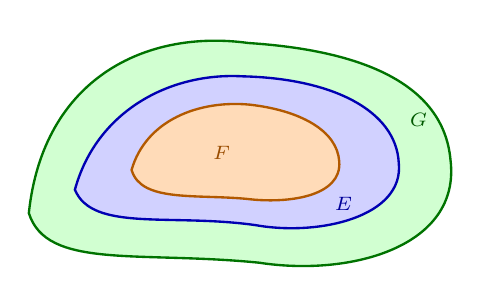
\begin{tikzpicture}[
  scale=0.90,
  every node/.style={font=\scriptsize},
  outerfill/.style={fill=green!18, draw=none},
  middlefill/.style={fill=blue!18, draw=none},
  innerfill/.style={fill=orange!28, draw=none},
  outerline/.style={draw=green!45!black, line width=0.85pt},
  middleline/.style={draw=blue!70!black, line width=0.85pt},
  innerline/.style={draw=orange!70!black, line width=0.85pt}
]
  \def\Outer{%
    (-3.0,-0.95)
      .. controls (-2.8,0.95) and (-1.35,1.65) .. (0.10,1.45)
      .. controls (1.65,1.35) and (2.85,0.90) .. (2.95,-0.20)
      .. controls (3.10,-1.42) and (1.55,-1.85) .. (0.25,-1.65)
      .. controls (-1.45,-1.48) and (-2.75,-1.75) .. (-3.0,-0.95)
      -- cycle%
  }
  \def\Middle{%
    (-2.35,-0.62)
      .. controls (-2.05,0.48) and (-1.02,1.04) .. (0.02,0.98)
      .. controls (1.28,0.95) and (2.18,0.50) .. (2.22,-0.24)
      .. controls (2.30,-1.00) and (1.10,-1.28) .. (0.20,-1.12)
      .. controls (-1.00,-0.95) and (-2.10,-1.22) .. (-2.35,-0.62)
      -- cycle%
  }
  \def\Inner{%
    (-1.55,-0.34)
      .. controls (-1.35,0.36) and (-0.60,0.65) .. (0.12,0.58)
      .. controls (0.82,0.50) and (1.35,0.22) .. (1.38,-0.22)
      .. controls (1.42,-0.72) and (0.65,-0.82) .. (0.08,-0.75)
      .. controls (-0.65,-0.68) and (-1.42,-0.80) .. (-1.55,-0.34)
      -- cycle%
  }

  \path[outerfill] \Outer;
  \path[middlefill] \Middle;
  \path[innerfill] \Inner;

  \draw[outerline] \Outer;
  \draw[middleline] \Middle;
  \draw[innerline] \Inner;

  \node[green!35!black] at (2.50,0.36) {$G$};
  \node[blue!60!black] at (1.44,-0.82) {$E$};
  \node[orange!60!black] at (-0.28,-0.10) {$F$};
\end{tikzpicture}

  \caption{Regular approximation sandwiches $E$ between $F$ and $G$ with small excess.}
  \label{fig:regular-approximation-sandwich}
\end{figure}

\begin{theorem} \label{thm:lebesgue-measurable-non-borel-sets-exist} \hlt{Lebesgue Measurable Non-Borel Sets Exist}
\begin{enumerate}[label=(\roman*)]
\setlength{\itemsep}{0pt}
\item There exists $E\subseteq\R$ such that $E\in\mathcal{L}^1$ and $E\notin\mathcal{B}(\R)$.
\item $\mathcal{B}(\R)\subsetneq\mathcal{L}^1$.
\end{enumerate}
\begin{proof}
\begin{enumerate}[label=(\roman*)]
\setlength{\itemsep}{0pt}
\item Lemma \ref{lem:open-sets-countable-unions-rational-boxes} gives $\abs{\mathcal{B}(\R)}\leq\mathfrak{c}$. Let $C$ be the Cantor set. Since $\abs{C}=\mathfrak{c}$ and $m(C)=0$, Proposition \ref{prop:outer-null-sets-lebesgue-measurable} gives $\mathcal{P}(C)\subseteq\mathcal{L}^1$, so $\abs{\mathcal{L}^1}\geq2^{\mathfrak{c}}>\mathfrak{c}$. Hence some $E\in\mathcal{L}^1$ is not Borel.
\item Proposition \ref{prop:borel-hierarchy-first-examples} gives $\mathcal{B}(\R)\subseteq\mathcal{L}^1$, and (i) makes the containment proper.
\end{enumerate}
\hlt{Structural Commentary}: Countable generation is smaller than completion by null subsets.\\
\hlt{Key Insight}: Completeness creates more measurable sets than topology can generate.
\end{proof}
\end{theorem}
